\documentclass[conference]{IEEEtran}

\usepackage{cite}
\usepackage{amsmath,amssymb}
\usepackage{graphicx}
\usepackage{booktabs}
\usepackage{placeins}
\usepackage{tikz}
\usetikzlibrary{arrows.meta,positioning,fit,calc}
\usepackage{url}
\usepackage[hidelinks]{hyperref}

\title{From Plausible Output to Engineering Practice:
Design Principles for Controlled AI-Supported Engineering}

\author{
\IEEEauthorblockN{Moritz Diez}
\IEEEauthorblockA{
Systems Engineering\\
Munich, Germany\\
}
}

\begin{document}

\maketitle

\begin{abstract}
Generative artificial intelligence is increasingly capable of supporting engineering
activities that involve the interpretation of heterogeneous, weakly structured, or
partially formalized information. However, the productive use of probabilistic AI in
engineering requires more than the generation of plausible technical content. Engineering
results must remain grounded in relevant source information, uncertainty must be made
visible, consequential decisions require explicitly assigned authority, and generated
artifacts need to remain traceable and independently verifiable.

This paper derives a set of design principles for controlled AI-supported engineering
from the development and investigation of an information-processing architecture for
the transformation of heterogeneous legacy engineering information into SysML v2.
The resulting principles address the definition of the engineering task and information
basis, probabilistic interpretation, uncertainty handling, human authority, constrained
downstream processing, provenance, traceability, and independent verification.

The paper further organizes these principles into a structured path toward productive use.
The proposed perspective is not intended as a prescriptive implementation method.
Instead, it identifies the questions and control boundaries that need to be addressed when
probabilistic AI is introduced into engineering workflows. The resulting view positions the
transition from AI experimentation to engineering practice primarily as a systems and
process design challenge rather than a prompting problem.

\end{abstract}

\begin{IEEEkeywords}
generative AI, systems engineering, human-in-the-loop, engineering authority,
provenance, traceability, technical validation
\end{IEEEkeywords}

\section{Introduction}

Generative artificial intelligence has expanded the range of engineering activities that
can be supported by automated information processing. Large language models can interpret
natural-language specifications, generate technical artifacts, support model creation, and
assist with the analysis of heterogeneous engineering information. Recent work has shown
both the potential of such approaches and their limitations in systems engineering and
model-based engineering contexts \cite{Topcu2025,Stein2026,Cibrian.2025}.

The introduction of generative AI into engineering workflows is nevertheless not equivalent
to the establishment of a reliable engineering process. Engineering information is often
distributed across heterogeneous legacy sources, differs in structure, terminology,
granularity, and abstraction level, and may evolve over time
\cite{Maheshwari2018,Henderson2024,Legat2014}. In such environments, technical access to
information does not by itself resolve the question of what the information means, how
reliable a particular interpretation is, or whether it may be used as the basis for a
subsequent engineering decision.

This distinction is particularly relevant for probabilistic AI. A generated result may be
linguistically convincing or formally valid while still containing engineering-relevant
errors or unsupported assumptions \cite{Topcu2025,Stein2026}. Consequently, the central
question is not only whether AI can produce engineering-related output, but under which
conditions such output can become part of a controlled engineering workflow.

The investigation underlying this paper addressed this problem in the context of a
controlled AI-supported transformation of heterogeneous legacy engineering information
into SysML v2. The developed architecture combined source-grounded information,
probabilistic interpretation, explicit human authorization, controlled downstream
transformation, provenance, traceability, and technical validation. Repeated transformation
runs were used to refine the boundaries between information processing, engineering
decision-making, and model formation.

Based on these findings and the literature used in the underlying investigation, this paper
derives generalized design principles for AI-supported engineering. The focus is deliberately
not placed on one particular technical implementation. Instead, the paper addresses the
questions that need to be resolved when probabilistic AI becomes part of an engineering
process: what information may support engineering statements, where interpretation is
required, how uncertainty is handled, where engineering authority resides, how processing
is constrained, and how resulting artifacts remain traceable and subject to assessment
distinct from their generation.

The remainder of the paper is structured as follows. Section II outlines the main challenges
of AI-supported engineering. Section III derives design principles for controlled use.
Section IV organizes these principles into a structured path toward productive engineering
application. Section V discusses transferability, context dependence, and limitations, and
Section VI concludes the paper.

\section{What Makes AI-Supported Engineering Difficult?}
\label{sec:challenges}

The use of generative AI in engineering differs from unconstrained content generation.
Engineering information contributes to technical decisions, system descriptions, models,
requirements, and other artifacts that may remain relevant throughout the system lifecycle.
AI-supported processing must therefore consider not only whether technically plausible
content can be generated, but also how the underlying information is interpreted, which
results may be used for subsequent engineering activities, and how the resulting states
remain verifiable and traceable.

\subsection{Engineering Task and Information Basis}
\label{sec:challenge_information_basis}

The introduction of AI support first requires a sufficiently bounded engineering task.
The intended result determines which source information is relevant, which interpretation
steps are required, and which criteria can later be used to assess the result. This becomes
particularly important in brownfield environments, where relevant system information may
already exist across specifications, tables, technical documents, models, or further data
sources \cite{Maheshwari2018,Henderson2024}.

Such information does not generally form a uniform or fully formalized basis. Sources may
differ in format, degree of structure, terminology, granularity, level of abstraction, and
currency. Several sources may describe the same system aspect from different perspectives,
complement each other, or contain diverging statements. The processing task therefore
cannot be reduced to making existing documents technically accessible.

A controlled AI-supported workflow also has to distinguish the role that available
information plays within the engineering task. In the underlying investigation,
\emph{Engineering Sources} formed the domain-specific information basis from which
statements about the system could be derived. \emph{Context Sources} provided additional
information for interpretation and classification without themselves constituting the
engineering evidence for the system under consideration. The \emph{Processing and
Orchestration Context}, including prompts, agent roles, and processing configurations,
influenced how information was processed but likewise did not establish engineering facts.

This distinction is relevant beyond the investigated transformation task. Information that
supports interpretation should not implicitly acquire the same authority as information
that constitutes the engineering basis itself. At the same time, the conditions under which
a result was generated remain relevant for understanding its origin. Provenance therefore
concerns both the source information and the processing context that contributed to the
result \cite{MoreauMissier2013,Simmhan2005}.

\subsection{Interpretation, Heterogeneity, and Uncertainty}
\label{sec:challenge_interpretation}

For formally defined source and target models, transformation can be governed by explicit
rules and metamodels. Heterogeneous legacy information introduces an additional problem:
before information can be transformed into a target structure, its engineering meaning has
to be identified and placed into the relevant system context.

The heterogeneity of engineering information is therefore not only a technical format
problem but also a semantic one. Information may only become understandable in relation to
its domain context, terminology, related artifacts, or existing engineering knowledge
\cite{Bressan.2000}. This
interpretation task is one area in which probabilistic AI can provide value, because it can
generate possible interpretations of weakly structured or natural-language information.

However, probabilistic interpretation introduces uncertainty. A linguistically convincing
or formally valid result does not provide direct evidence of engineering correctness.
Studies of LLM-generated systems-engineering artifacts have shown that outputs resembling
expert artifacts can still contain technically relevant errors or unsupported assumptions
\cite{Topcu2025}. Related approaches to model generation therefore combine generative
processing with intermediate representations, additional constraints, or validation
mechanisms \cite{Cibrian.2025,Stein2026,Pan.2025}.

The underlying investigation addressed this problem by applying several configured
perspectives to the same source-grounded engineering subject. Agreement between
interpretations provided information about \emph{Consensus}, while relevant differences
were represented as \emph{Variance}. A situation in which several perspectives identified
the same unresolved information or ambiguity was represented as \emph{Shared Ambiguity}.
Such multi-perspective processing can provide additional evidence for subsequent evaluation,
but agreement alone does not establish that an interpretation is correct
\cite{Du2024,TriemDing2024}.

The more general implication is that uncertainty should remain visible within an
AI-supported engineering process. Missing information, conflicting interpretations, or
insufficient evidence should not automatically be converted into apparently complete
engineering information by generative processing.

\subsection{Engineering Authority and Controlled Processing}
\label{sec:challenge_authority}

Probabilistic interpretation and engineering decision-making represent different functions.
AI-generated interpretations can provide decision support, but the decision whether a
particular interpretation may be used for subsequent engineering activities has a different
status.

Human-in-the-loop approaches describe different forms of human participation, ranging from
supervision and feedback to explicit evaluation and decision-making
\cite{MosqueiraRey2023,Lazaros2026}. In the investigated architecture, human involvement
was therefore represented as explicit decision authority at defined transitions of the
engineering process.

The \emph{Human Engineering Authority} authorized the domain-specific use of interpreted
engineering information. This decision referred to a defined information state rather than
to an abstract source or an unrestricted AI output. A materially changed state therefore
required a new evaluation.

A separate \emph{Model Authority} addressed a different decision object: how already
authorized engineering information should be structurally placed and represented in the
target model. This distinction emerged from the observation that engineering meaning,
structural representation, and target-specific formulation are not necessarily identical
decisions.

The exact authority roles depend on the engineering task. The general challenge is to avoid
allowing probabilistic processing to implicitly determine consequential engineering states.
Once the required engineering meaning, authority, and representation rules have been
resolved, subsequent processing can increasingly rely on explicit rules and constraints.
Conversely, if the required evidence, authorization, or transformation rule is missing, the
unresolved state should remain visible rather than being silently completed by the AI
system.

\subsection{Traceability, Assurance, and Integration}
\label{sec:challenge_assurance}

AI-supported engineering creates a chain of information states rather than a single
generation event. Source information may be identified, interpreted, evaluated, authorized,
transformed, and finally represented in a technical artifact. If only the final artifact is
retained, the relationship between the result and the decisions that produced it is lost.

Provenance describes the origin and derivation of information
\cite{MoreauMissier2013,Simmhan2005}. Traceability connects the resulting information,
decision, and artifact states \cite{ISO29148}. In the underlying investigation, source-grounded evidence,
AI-generated interpretations, human authorization decisions, intermediate model states,
and the final artifact remained explicitly connected. This allowed the processing path to
be reconstructed from source to result and, conversely, from a resulting model element back
to its underlying information and decisions.

This becomes increasingly relevant when several Engineering Sources contribute to a common
engineering result. Related information may need to be considered jointly while the
individual origin and authorization state of each contribution remain distinguishable.

Finally, generation and the subsequent assessment of the resulting artifact address
different questions. The fact that an AI system can produce an artifact does not demonstrate
that the artifact satisfies the relevant engineering, formal, or technical criteria.
Appropriate assessment mechanisms therefore have to be defined separately from the
generation step \cite{Topcu2025,Cibrian.2025,Stein2026}.

Moving from a bounded AI-supported task toward productive engineering use adds an
organizational dimension. The workflow has to be integrated into existing responsibilities,
quality mechanisms, and engineering processes. In addition, increasing processing volume
also increases the need to consider the scalability of human review and authorization.
These questions extend beyond model capability and make productive AI-supported engineering
a combined information, process, and systems-engineering challenge.

\section{Design Principles for Controlled AI-Supported Engineering}
\label{sec:design_principles}

The challenges described in Section~\ref{sec:challenges} can be translated into a set of
design principles for controlled AI-supported engineering. These principles do not define
one universal implementation architecture. Instead, they describe boundaries and control
mechanisms that proved relevant in the underlying investigation. Their potential
transferability to comparable engineering tasks is discussed in
Section~\ref{sec:discussion_transferability}.

\subsection{Start from the Engineering Task}
\label{sec:principle_task}

AI support should be designed around a sufficiently bounded engineering task. The intended
engineering result defines which information is relevant, which interpretation steps are
necessary, and which acceptance criteria can later be applied.

This task orientation is important because an AI model does not define the engineering
process in which its output will be used. The same model may support fundamentally different
activities, from information extraction to requirements analysis or model generation.
Consequently, the engineering purpose, expected output, and boundaries of AI support need to
be defined before technical implementation choices are made.

A bounded task also creates the basis for later decisions about information authority,
human review, verification, and acceptable automation.

\subsection{Establish a Controlled Information Basis}
\label{sec:principle_information_basis}

AI-supported engineering should operate on an explicitly defined information basis. The
relevant question is not only which information is available, but also which information may
justify engineering statements and which information merely supports their interpretation.

The investigated architecture therefore distinguished between \emph{Engineering Sources},
\emph{Context Sources}, and the \emph{Processing and Orchestration Context}. This distinction
made it possible to separate source-grounded evidence from information that
supported interpretation or influenced processing.

The exact source taxonomy depends on the engineering task. The general principle is that
different information roles should remain explicit and should not silently inherit the same
engineering authority. At the same time, information required to understand how a result was
produced should remain available as provenance.

\subsection{Use Probabilistic AI Where Interpretation Is Required}
\label{sec:principle_probabilistic}

Probabilistic AI is particularly useful where engineering information cannot be transformed
through explicit rules alone and instead requires semantic interpretation.

This situation occurs when source information is weakly structured, expressed in natural
language, uses inconsistent terminology, or can only be understood in relation to wider
domain context. In such cases, probabilistic processing can generate candidate
interpretations and thereby provide information for a subsequent engineering decision.

Where source and target semantics are already sufficiently formalized, however, additional
probabilistic processing may add unnecessary variability. Formal model-transformation
approaches demonstrate that explicit transformation rules can provide deterministic behavior
where the required relationships are already known \cite{Kapos.2014,Li.2022,Zhou.2024}.

The resulting principle is therefore not to maximize AI usage, but to place probabilistic
processing at those points where interpretation is actually required.

\subsection{Make Uncertainty Explicit}
\label{sec:principle_uncertainty}

Probabilistic processing should not convert uncertainty into apparently complete engineering
information without making the unresolved state visible.

In the underlying investigation, several configured perspectives were used to expose
different interpretation outcomes. Agreement could be represented as \emph{Consensus},
differences as \emph{Variance}, and jointly recognized unresolved information as
\emph{Shared Ambiguity}. These states provided additional information for subsequent human
evaluation.

The specific mechanism is not essential to the general principle. Multiple AI perspectives
represent one possible way to expose uncertainty, but other workflows may use confidence
indicators, contradiction detection, explicit unknown states, or targeted review triggers.

The important distinction is that uncertainty should remain part of the engineering state.
Agreement may strengthen the evidence available for a decision, but does not by itself prove
engineering correctness. Likewise, missing information should remain identifiable as missing
rather than being completed solely because a generative system can produce a plausible
continuation.

\subsection{Keep Engineering Authority Explicitly Assigned}
\label{sec:principle_authority}

AI-generated interpretations can support engineering decisions without themselves acquiring
engineering authority.

In the investigated architecture, the \emph{Human Engineering Authority} decided whether a
defined interpretation state could be used as authorized engineering information. A separate
\emph{Model Authority} addressed the structural placement and representation of already
authorized content in the target model.

This separation emerged because engineering meaning and model representation constituted
different decision objects. A statement may be accepted as technically meaningful without
this automatically determining how it should be represented in a model or downstream
artifact.

The exact authority roles are context dependent. Some engineering tasks may require fewer
decision boundaries, while others may require additional domain, quality, or release
authorities. The transferable principle is that consequential state transitions should have
an explicitly assigned decision authority instead of allowing probabilistic processing to
implicitly determine their outcome.

Authorization should refer to a clearly identifiable information state. If that state is
materially changed, the previous authorization should not automatically be assumed to remain
valid.

\subsection{Constrain Downstream Processing Once Decisions Are Resolved}
\label{sec:principle_constraints}

Once the relevant engineering meaning, decision authority, and representation rules are
sufficiently resolved, subsequent processing should become increasingly rule-bound and
reproducible.

The investigated architecture used this separation to avoid repeated probabilistic
reinterpretation of already authorized information. Authorized engineering content was
carried forward into a controlled engineering state and processed through explicit modeling
and transformation rules before the final artifact was produced.

This principle reduces the number of points at which probabilistic behavior can change an
already established engineering decision. It also improves the ability to reproduce and
verify downstream processing.

A related consequence is fail-closed behavior. If required evidence, authorization, or a
necessary transformation rule is missing, processing should expose the unresolved condition
rather than silently infer a continuation. This does not imply that every workflow must stop
at the same type of event. It means that unresolved engineering decisions should not be
hidden by automatic completion.

\subsection{Preserve Provenance and Traceability}
\label{sec:principle_traceability}

Controlled AI-supported engineering requires more than storing the final result. The
relationships between source information, AI-generated interpretations, human decisions,
intermediate engineering states, and resulting artifacts should remain reconstructable.

Provenance describes where information originates and how it was derived
\cite{MoreauMissier2013,Simmhan2005}. For AI-derived interpretations, this also includes
the relevant processing conditions under which they were produced. Traceability connects
the relevant engineering states and decision objects throughout the workflow. Together, they make it possible to determine
why a result exists, which information contributed to it, and which decisions authorized its
use.

This becomes particularly important in multi-source scenarios. Information from several
Engineering Sources may contribute to one resulting engineering state, but integration
should not remove the ability to identify the individual source contribution and its
associated decision history.

Persisted intermediate states also support change analysis. If a source changes, affected
interpretations, decisions, and downstream artifacts can be identified rather than treating
the final result as an isolated output.

\subsection{Assess Results Separately from Their Generation}
\label{sec:principle_verification}

Generation and the subsequent assessment of the resulting engineering artifact should
remain distinct functions.

An AI system may produce a syntactically plausible or formally valid artifact while the
artifact still contains engineering-relevant errors, incomplete relationships, or unsupported
content \cite{Topcu2025,Cibrian.2025,Stein2026}. The fact that the generation process
completed successfully is therefore not sufficient evidence that the result satisfies its
engineering purpose.

The required assessment mechanisms should instead be selected according to the target
artifact and the engineering task. Depending on the application, this may include syntax
checks, structural validation, semantic constraints, consistency checks, model-tool
validation, human model review, or further domain-specific acceptance criteria.

The investigated architecture treated technical validation, human model review, and final release
as distinct concerns. This separation prevents successful generation from being interpreted
as automatic approval and creates an explicit assurance boundary before the resulting
artifact is used in subsequent engineering work.

Taken together, these principles describe a controlled division of responsibilities:
probabilistic AI supports interpretation where ambiguity exists; engineering authority
governs consequential decisions; rule-bound processing handles sufficiently determined
states; provenance and traceability preserve the processing history; and separate
assessment provides evidence about the resulting artifact.

\section{A Structured Path Toward Productive Use}
\label{sec:path}

The design principles described in Section~\ref{sec:design_principles} can be organized
into a structured sequence for designing an AI-supported engineering workflow. The
sequence is not intended as a universal implementation lifecycle. Its purpose is to make
the main engineering questions explicit before probabilistic AI is integrated into a
productive process.

Figure~\ref{fig:controlled_ai_workflow} summarizes this processing logic. It abstracts the
architecture investigated in the underlying work into a sequence from source-grounded
information through probabilistic interpretation and explicit engineering authority to a
controlled engineering state and a verified engineering artifact.

\begin{figure*}[t]
\centering

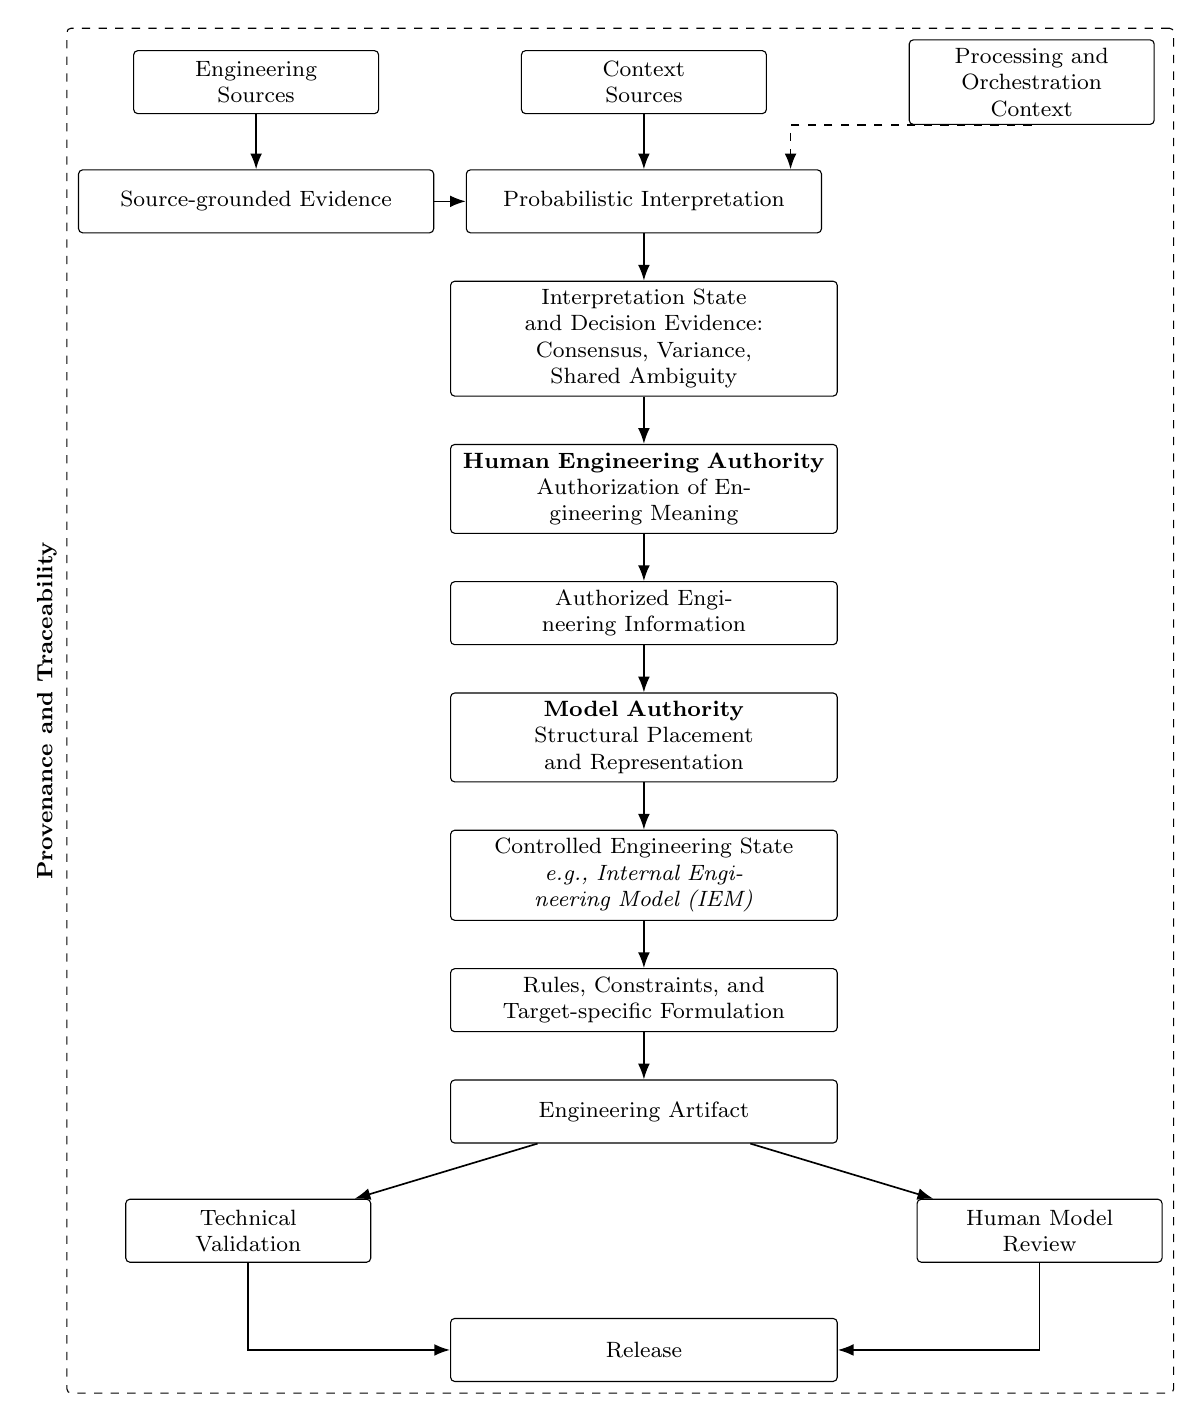
\begin{tikzpicture}[
    font=\footnotesize,
    node distance=6mm and 7mm,
    box/.style={
        draw,
        rounded corners=1.5pt,
        align=center,
        minimum height=8mm,
        text width=34mm,
        inner sep=3pt
    },
    smallbox/.style={
        draw,
        rounded corners=1.5pt,
        align=center,
        minimum height=8mm,
        text width=29mm,
        inner sep=3pt
    },
    widebox/.style={
        draw,
        rounded corners=1.5pt,
        align=center,
        minimum height=8mm,
        text width=47mm,
        inner sep=3pt
    },
    arrow/.style={
        -{Latex[length=2mm]},
        line width=0.6pt
    },
    influence/.style={
        -{Latex[length=2mm]},
        line width=0.6pt,
        dashed
    },
    span/.style={
        draw,
        dashed,
        rounded corners=1.5pt,
        inner sep=4pt
    }
]

% ------------------------------------------------------------------
% Information basis
% ------------------------------------------------------------------

\node[smallbox] (engsource)
    {Engineering\\Sources};

\node[smallbox, right=18mm of engsource] (contextsource)
    {Context\\Sources};

\node[smallbox, right=18mm of contextsource] (processingcontext)
    {Processing and\\Orchestration Context};

\node[widebox, text width=43mm, below=7mm of engsource] (evidence)
    {Source-grounded Evidence};

\node[widebox, text width=43mm, below=7mm of contextsource] (interpretation)
    {Probabilistic Interpretation};

\draw[arrow] (engsource) -- (evidence);

\draw[arrow] (evidence.east) -- (interpretation.west);

\draw[arrow]
    (contextsource.south)
    -- (interpretation.north);

\draw[influence]
    (processingcontext.south)
    -| ($(interpretation.north east)+(-4mm,0)$);

% ------------------------------------------------------------------
% Interpretation outcome
% ------------------------------------------------------------------

\node[widebox, below=6mm of interpretation] (uncertainty)
    {Interpretation State and Decision Evidence:\\
     Consensus, Variance, Shared Ambiguity};

\node[widebox, below=6mm of uncertainty] (hea)
    {\textbf{Human Engineering Authority}\\
     Authorization of Engineering Meaning};

\node[widebox, below=6mm of hea] (authorized)
    {Authorized Engineering Information};

\draw[arrow] (interpretation) -- (uncertainty);
\draw[arrow] (uncertainty) -- (hea);
\draw[arrow] (hea) -- (authorized);

% ------------------------------------------------------------------
% Model / representation authority
% ------------------------------------------------------------------

\node[widebox, below=6mm of authorized] (modelauthority)
    {\textbf{Model Authority}\\
     Structural Placement and Representation};

\node[widebox, below=6mm of modelauthority] (controlled)
    {Controlled Engineering State\\
     \emph{e.g., Internal Engineering Model (IEM)}};

\node[widebox, below=6mm of controlled] (rules)
    {Rules, Constraints, and\\
     Target-specific Formulation};

\node[widebox, below=6mm of rules] (artifact)
    {Engineering Artifact};

\draw[arrow] (authorized) -- (modelauthority);
\draw[arrow] (modelauthority) -- (controlled);
\draw[arrow] (controlled) -- (rules);
\draw[arrow] (rules) -- (artifact);

% ------------------------------------------------------------------
% Assessment and release
% ------------------------------------------------------------------

\node[smallbox, below left=7mm and 10mm of artifact] (validation)
    {Technical\\Validation};

\node[smallbox, below right=7mm and 10mm of artifact] (review)
    {Human Model\\Review};

\coordinate (assessmentmid)
    at ($(validation.south)!0.5!(review.south)$);

\node[widebox, below=7mm of assessmentmid] (release)
    {Release};

\draw[arrow] (artifact) -- (validation);
\draw[arrow] (artifact) -- (review);

\draw[arrow] (validation.south) |- (release.west);
\draw[arrow] (review.south) |- (release.east);

% ------------------------------------------------------------------
% Cross-cutting provenance and traceability
% ------------------------------------------------------------------

\node[
    span,
    fit=(engsource)(processingcontext)(evidence)(interpretation)
        (uncertainty)(hea)(authorized)(modelauthority)
        (controlled)(rules)(artifact)(validation)(review)(release),
    label={[rotate=90,anchor=south]west:
        \textbf{Provenance and Traceability}}
] (tracebox) {};

\end{tikzpicture}

\caption{Generalized processing structure for controlled AI-supported engineering.
Engineering Sources provide the basis for source-grounded evidence, while Context Sources
support interpretation and the Processing and Orchestration Context influences how the
interpretation is produced. Probabilistic outputs remain decision evidence until explicitly
authorized. The Internal Engineering Model (IEM) illustrates one implementation of the more
general controlled engineering state.}
\label{fig:controlled_ai_workflow}
\end{figure*}


Table~\ref{tab:key_questions} condenses the corresponding design questions and their
implications for an AI-supported engineering workflow.

\begin{table*}[t]
\caption{Key Questions for Designing AI-Supported Engineering Workflows}
\label{tab:key_questions}
\centering
\renewcommand{\arraystretch}{1.15}
\begin{tabular}{p{0.12\textwidth} p{0.35\textwidth} p{0.43\textwidth}}
\toprule
\textbf{Area} &
\textbf{Key Question} &
\textbf{Design Implication} \\
\midrule

Task &
What engineering outcome is required? &
Bound the engineering task, expected result, and acceptance criteria. \\

Information &
Which information may justify an engineering statement? &
Distinguish Engineering Sources from contextual and processing information. \\

Interpretation &
Where is semantic interpretation required? &
Use probabilistic processing where explicit transformation rules are insufficient. \\

Uncertainty &
What happens when information is ambiguous, incomplete, or contradictory? &
Preserve unresolved states rather than silently completing them. \\

Authority &
Who decides whether an interpretation may be used for subsequent engineering work? &
Assign explicit engineering authority at consequential transitions. \\

Processing &
Which downstream decisions are already sufficiently determined? &
Apply explicit rules and constraints instead of repeated probabilistic interpretation. \\

Traceability &
Why does a resulting engineering state exist? &
Connect sources, interpretations, decisions, intermediate states, and artifacts. \\

Assurance &
How is the resulting artifact assessed? &
Keep generation distinct from technical validation, human review, and release. \\

\bottomrule
\end{tabular}
\end{table*}


\subsection{Define the Engineering Task and Intended Result}
\label{sec:path_task}

The starting point is the engineering task rather than the AI technology. The intended
result, the boundaries of the task, and the criteria by which the result will later be
assessed need to be defined first.

This establishes the basis for all subsequent decisions. Without a sufficiently bounded
task, it remains unclear which information is relevant, where interpretation is required,
which decisions have engineering consequences, and which form of verification is
appropriate.

The task definition should therefore clarify at least the engineering purpose, the
expected result, the scope of AI support, and the conditions under which the result can be
considered usable for subsequent engineering activities.

\subsection{Establish the Information Basis}
\label{sec:path_information}

The next step is to identify the information on which the engineering task may rely.
Available information should not only be collected but classified according to its role
within the workflow.

The underlying investigation distinguished \emph{Engineering Sources}, \emph{Context
Sources}, and the \emph{Processing and Orchestration Context}. This separation made it
possible to distinguish information that could support statements about the system from
information that supported interpretation or influenced the processing procedure.

For another engineering task, the exact classification may differ. The relevant question
remains which information may justify an engineering statement and which information is
used only to interpret, structure, or process it.

\subsection{Identify Where Interpretation Is Required}
\label{sec:path_interpretation}

Once the information basis is known, the workflow can distinguish between information that
can be processed through explicit rules and information that requires semantic
interpretation.

Probabilistic AI is particularly useful at the latter boundary. Natural-language
descriptions, incomplete structures, inconsistent terminology, and different abstraction
levels can require interpretation before they can be integrated into a controlled
engineering state.

The purpose of AI processing at this stage is not to replace the engineering decision but
to provide interpretable candidates and supporting evidence for that decision.

\subsection{Make Unresolved Information Explicit}
\label{sec:path_uncertainty}

Probabilistic interpretation may produce agreement, competing interpretations, incomplete
information, or unresolved ambiguity. These conditions should remain visible in the
processing state.

In the underlying architecture, \emph{Consensus}, \emph{Variance}, and
\emph{Shared Ambiguity} represented different outcomes of multi-perspective interpretation.
Other implementations may use different mechanisms, but the underlying requirement
remains the same: unresolved information should not disappear merely because a generative
system is able to formulate a plausible continuation.

This step therefore defines how ambiguity, contradiction, missing information, and
insufficient evidence are represented and under which conditions further processing is
blocked or escalated.

\subsection{Assign Engineering Authority}
\label{sec:path_authority}

Where AI-generated interpretations can influence subsequent engineering work, the workflow
needs an explicit decision boundary.

In the investigated architecture, the \emph{Human Engineering Authority} decided whether
an interpretation state could be used as authorized engineering information. Where a
subsequent structural representation decision was required, the \emph{Model Authority}
addressed that separate decision.

The exact role structure depends on the engineering task. The central requirement is that
the transition from a probabilistic interpretation to an authorized engineering state is
explicit and attributable to a defined authority.

Authorization should refer to a clearly identifiable state. If the underlying information
or interpretation changes materially, the corresponding decision state has changed as
well.

\subsection{Create a Controlled Engineering State}
\label{sec:path_controlled_state}

After the relevant interpretation and authority decisions have been resolved, downstream
processing should no longer depend directly on unrestricted AI output.

Instead, the authorized content can be transferred into a controlled engineering state
that provides a stable basis for subsequent processing. In the underlying implementation,
this function was realized by the \emph{Internal Engineering Model} (IEM). The specific
representation is implementation-dependent; the more general requirement is to separate
authorized engineering information from the probabilistic processing that produced its
candidate interpretation.

This boundary allows downstream processing to operate on explicit identities, relations,
rules, and approved engineering content rather than repeatedly reinterpreting the original
source material.

\subsection{Apply Rules, Constraints, and Verification}
\label{sec:path_rules}

Once the decision space has been sufficiently resolved, transformation should become
rule-bound wherever appropriate. Target-specific constraints, representation rules, and
technical validation can then be applied to the controlled engineering state.

If the required evidence, authority, or rule is missing, the unresolved condition should
remain visible. A fail-closed transition prevents the workflow from silently introducing
new engineering meaning during downstream processing.

Generation and verification remain separate concerns. The resulting artifact should be
checked using mechanisms appropriate to its purpose and representation. Depending on the
engineering task, this can include structural validation, semantic constraints, consistency
checks, tool-based validation, human review, and release criteria.

\subsection{Preserve Traceability and Integrate the Workflow}
\label{sec:path_integration}

The complete processing path should remain reconstructable from the original information
basis through interpretation and human decisions to the resulting engineering artifact.
Provenance and traceability therefore span all preceding steps rather than forming a final
documentation activity.

For multi-source workflows, this also requires preserving source-local provenance when
information is integrated into a common engineering state.

The final step toward productive use is organizational integration. Responsibilities,
review activities, quality gates, and release mechanisms need to fit the existing
engineering process. Increasing the scope of AI support also requires evaluating whether
the associated review and authorization effort remains practicable.

The resulting sequence can therefore be understood as a transition from probabilistic
interpretation to controlled engineering use: source information is interpreted where
necessary, consequential decisions remain explicitly authorized, authorized content is
transferred into a controlled state, downstream processing becomes increasingly
rule-bound, and the resulting artifact remains traceable and independently verifiable.

\section{Discussion}
\label{sec:discussion}

The principles derived in the preceding sections originate from the development and
investigation of a controlled transformation architecture for heterogeneous legacy
engineering information into SysML v2. Their relevance beyond this specific application
therefore needs to be distinguished from those aspects that remain bound to the investigated
engineering task.

\subsection{Transferability and Context Dependence}
\label{sec:discussion_transferability}

Several mechanisms investigated in the underlying architecture are not inherently tied to
SysML v2 as a target representation. Source processing, provenance, stable identities,
persisted processing states, probabilistic interpretation, and explicit human authorization
address more general problems that also occur in other information-centered engineering
tasks.

This provides a basis for considering similar mechanisms in workflows such as requirements
review, technical-documentation analysis, or quality and regulatory documentation review.
Such tasks likewise involve heterogeneous documents that have to be interpreted in relation
to an engineering context and whose resulting assessments may require explicit human
decisions.

The transferability of these mechanisms should nevertheless be understood as a further
hypothesis rather than as an empirically demonstrated property across engineering domains.
The underlying investigation was limited to a specific brownfield transformation task and
to a defined SysML-v2 target.

In particular, task-specific aspects cannot simply be transferred unchanged. The relevant
Engineering Sources and Context Sources, the perspectives used for probabilistic
interpretation, the authority boundaries, the controlled engineering state, the
target-specific rules, and the assessment mechanisms all depend on the engineering
purpose.

The resulting distinction is important. A potentially transferable aspect is not one fixed
workflow configuration, but the separation of functions: controlled source processing,
probabilistic interpretation, explicit engineering decisions, persistent states,
rule-bound downstream processing, provenance, traceability, and separate assessment.

\subsection{From Controlled Prototype to Productive Engineering Use}
\label{sec:discussion_productive_use}

The investigated architecture demonstrates a controlled processing path under bounded
conditions. Productive use introduces additional questions that were only addressed to a
limited extent in the underlying work.

A first challenge concerns the information basis itself. Productive environments contain
larger and less curated information sets, additional document types, changing information
states, and potentially broader sets of engineering constructs. The mechanisms for source
classification, interpretation, authorization, and controlled integration therefore need to
remain effective as the amount and diversity of information increase.

A second challenge concerns human review. Explicit authorization provides a control
boundary, but it also creates review effort. As the processing volume increases, the
scalability of human review and authorization becomes part of the engineering problem.
The relevant question is therefore not whether the human expert should be removed from the
process, but how human attention can be focused on those states in which engineering
judgement is actually required.

A third challenge is the integration into an existing engineering workflow. Domain
references, interpretation perspectives, rules, representation frameworks, review
responsibilities, and release mechanisms need to fit the respective organizational
context. The practical quality of such a workflow therefore depends not only on model
performance but also on the comprehensibility of the provided decision basis, the actual
review effort, and the compatibility of the authority boundaries with established working
practices. Prior work on MBSE adoption likewise highlights the relevance of organizational
context, perceived value, and adoption conditions when engineering methods are introduced
into practice \cite{Henderson2024,Call2022,Campo2023,Nanfuka2023}.

Finally, productive use also requires the conventional qualities expected from an
engineering software system. Software quality, runtime behavior, resource demand,
robustness, maintainability, and operational integration remain relevant independently of
the AI-specific architecture.

These aspects reinforce the main observation of this paper: moving from an AI-supported
demonstrator to productive engineering use is not merely a matter of improving the
underlying model. The information basis, decision boundaries, engineering rules,
assessment mechanisms, and organizational workflow have to evolve together.

\subsection{Learning from Human Engineering Decisions}
\label{sec:discussion_learning}

Persisted human decisions create an additional long-term perspective. Over repeated use,
an AI-supported engineering workflow can accumulate a structured data basis that connects
engineering information, machine-generated proposals, and the corresponding human
evaluations or corrections.

Research on learning from human feedback demonstrates that human evaluations can provide
useful learning signals for adaptive systems \cite{Christiano2017,Ouyang2022}. In an
engineering context, however, such feedback remains meaningful only if it can be related to
the information state and decision context from which it originated.

The provenance and state persistence required for traceability can therefore also provide
a basis for controlled learning. Repeated corrections may indicate that interpretation
instructions, examples, rules, or specialized models should be adapted. Such adaptations
should themselves be versioned, evaluated separately, and explicitly released before they
become part of the productive workflow.

With increasing quality of machine-generated interpretations, human review may eventually
be concentrated more strongly on cases characterized by relevant uncertainty, variance,
contradictory information, or novel situations. Whether individual decisions can be further
automated should, however, be determined empirically from future application data rather
than assumed from model capability alone.

This perspective extends the architecture from a controlled transformation process toward
a potentially adaptive engineering workflow while retaining the same fundamental
requirement: changes in automated behavior must remain attributable, assessable, and
subject to explicit engineering control.

\section{Conclusion}
\label{sec:conclusion}

This paper examined how probabilistic AI can be integrated into engineering workflows
while preserving explicit engineering decision authority and the traceability of the
resulting information states.

A central finding of the underlying investigation is the need to separate different processing and decision functions.
Probabilistic methods can make heterogeneous information accessible and provide alternative
interpretations as a basis for subsequent evaluation. Engineering meaning, structural
representation, and target-specific formulation may constitute different decision objects.
Consequential transitions therefore require explicitly assigned engineering authority,
while processing can become increasingly rule-bound once the relevant decisions have been
resolved.

Provenance and traceability form cross-cutting functions throughout this process. Source
information, source-grounded evidence, machine-generated interpretations, human
authorization decisions, controlled engineering states, and resulting artifacts should
remain identifiable and connected. This allows the development of an engineering result to
be reconstructed from its information basis and, conversely, allows a resulting artifact
to be traced back to the information and decisions on which it depends.

The findings therefore suggest that controlled AI support depends on the interaction of
probabilistic interpretation, explicit human authorization, semantic and engineering
constraints, rule-bound technical processing, technical validation, human review, and
release. None of
these mechanisms alone establishes a controlled engineering process.

The transition from AI experimentation to productive engineering use is consequently not
primarily a prompting problem. It is a systems and process design challenge in which the
information basis, uncertainty handling, decision authority, technical constraints,
traceability, assessment, and integration into existing engineering workflows have to be
considered together.


\bibliographystyle{IEEEtran}
\bibliography{references}

\end{document}
